% zitex: arXiv manuscript. Build with XeLaTeX, twice:   xelatex main.tex
% The folder is self-contained: zitex.sty, fonts.yaml and zitex-out/ (the snippets) were made by
%   zitex setup -o . ; zitex extract -c 器,藻,佛 -o .     and this file replaces the generated main.tex.
% The picture-row examples (section 4) were added with
%   zitex render -i chars.yaml --scan main.tex -x lexicon.yaml -x obs/lexicon.yaml -l en -l zh
% where obs/ holds the oracle bone glyphs (exported from Orascope; HUST-OBC, CC BY-NC 4.0).
\documentclass[11pt]{article}
\usepackage[margin=2.4cm]{geometry}
\usepackage{zitex}% sets a CJK font: Noto Serif CJK SC, or FandolSong from TeX Live if that is not installed
% The submission carries a subset of Noto Serif CJK SC (SIL OFL 1.1), so the glyphs are the same on any machine:
\IfFileExists{fonts/NotoSerifCJKsc-Subset-Regular.otf}{%
  \setCJKmainfont{NotoSerifCJKsc-Subset-Regular.otf}[Path=fonts/, BoldFont=NotoSerifCJKsc-Subset-Bold.otf]}{}
\usepackage{booktabs}
\usepackage{graphicx}
\usepackage{caption}
\usepackage[hidelinks]{hyperref}
\captionsetup{font=small,labelfont=bf}
\setlength{\emergencystretch}{2em}
\newcommand{\cmd}[1]{\texttt{\textbackslash #1}}

\title{Decomposing Chinese Characters:\\ \LaTeX{} Typesetting with \texttt{zitex}}
\author{Wen G. Gong\\ \texttt{wen.gong.research@gmail.com}}
\date{}

\begin{document}
\maketitle

\begin{abstract}
Chinese characters began as pictographs, as the oracle bone script shows, and every character has a sound, a shape and a meaning.
Presenting the three together and consistently is manual work today: pinyin and glosses are placed by hand, pictures are pasted and
aligned, decompositions are drawn in a graphics program, and none of it is tied to the data behind it. We present \texttt{zitex}, an
extension for XeLaTeX that makes the figure a function of the data. A character is a short entry giving its decomposition and the position
of each part in the eleven-position Zi-Matrix notation. A Python program validates the data and writes a self-contained snippet per
character and view: a one-line formula, a typeset equation with pinyin and glosses, a nested-box matrix, or a tree. A further view adds a
row of pictures under the meanings (an oracle bone glyph, an image or an emoji), so that each part shows its sound, its shape and its
meaning in rows that line up. A short \LaTeX{} package only includes those snippets. We describe the notation, the design, the handling
of fonts and of the source database, and the limits of the present version. \texttt{zitex} is released under the MIT licence at
\url{https://github.com/digital-duck/zinets-latex}.
\end{abstract}

\section{Introduction}
Chinese characters originated as pictographs. The oracle bone script, carved on turtle shells and animal bones in the late Shang dynasty more than
three thousand years ago, still shows the pictures: the sun is a circle, the moon a crescent, and a creature or a tool is drawn as what it is.
Modern characters have kept the sound and the meaning but lost most of the picture, which is why teachers and researchers keep placing the ancient
glyph next to the modern character.

Every character therefore has three dimensions: a sound (pinyin), a shape (the glyph, and how it is built from parts) and a meaning. Papers and teaching
material on characters need to present all three together, for each part of a character and for the character itself. Today this is manual work.
Pinyin and glosses are placed above and below the characters by hand, pictures are pasted and aligned one by one, and the decomposition is drawn in a graphics
program or in TikZ. The result is slow to produce, differs from one figure to the next, and must be redone when the underlying analysis changes. The
problem we address is a typesetting problem: to present Chinese characters with sound, shape and meaning in a consistent layout, generated and not made by hand.

A Chinese character can be read as the product of a reaction in which its parts go in and the character comes out, for example
\ziformula{佛}\unskip. This view is used to teach characters, to study how the writing system is organised, and to analyse its
structure computationally~\cite{gong2025}. We build on it: a character is a record, and the figure, in any of several views, is generated from the record.

This paper describes \texttt{zitex}, which typesets decompositions directly from data. Its aims are: (i) a figure is generated
from a record, so that revising the record revises the figure; (ii) the notation records \emph{where} each part sits, which
a flat sequence of components does not; (iii) sound, shape and meaning are laid out the same way for every character, in rows that line up, with
the shape given by an oracle bone glyph, an image or an emoji; (iv) the \LaTeX{} side stays small, and the data and layout logic live in
a program that can be tested; and (v) the source database is never modified. Section~\ref{sec:example} shows the oracle bone glyphs of 日, 月, 明, 虫, 工 and 虹
set next to their sounds and meanings.

\section{Notation}
A character is described level by level. At each level the parts have positions from a fixed set of eleven codes.

\begin{table}[ht]
\centering\small
\begin{tabular}{@{}ll@{}}
\toprule
Code & Region \\
\midrule
\texttt{L}, \texttt{R}, \texttt{U}, \texttt{D} & left, right, up, down \\
\texttt{LU}, \texttt{LD}, \texttt{RU}, \texttt{RD} & the four corners \\
\texttt{M} & the centre of gravity of the level \\
\texttt{Mi}, \texttt{Mo} & inside and outside (enclosing) \\
\bottomrule
\end{tabular}
\caption{The Zi-Matrix position codes, introduced in~\cite{gong2025}.}
\label{tab:codes}
\end{table}

The \emph{pattern} of a level is its position codes in reading order, such as \texttt{L-M} for 佛 or
\texttt{LU-RU-M-LD-RD} for 器. A pattern determines the matching Unicode ideographic description operator where one exists:
for instance \texttt{L-M} and \texttt{L-R} map to the left--right operator, and the enclosing patterns \texttt{Mo-D},
\texttt{Mo-U}, \texttt{Mo-R} and \texttt{Mo-M} map to the surrounding operators. Some arrangements have no single operator,
for example four mouths around a dog in 器. For these \texttt{zitex} adds a few operators (such as ∴ ∵ ∷) and a general form
that names the pattern. A \emph{radical rule} resolves the ambiguity of two-part levels: a Kangxi radical is peripheral, so the
radical is placed at \texttt{L} and the other part at \texttt{M}, as in 佛 (亻 and 弗). Positions are stored on every level, so a
part that is itself decomposed (澡 inside 藻) carries its own pattern.

\section{Design}
Python does the parsing and layout, and \LaTeX{} does the typesetting (Figure~\ref{fig:flow}). \texttt{zitex extract} selects characters
from a database and writes \texttt{chars.yaml}, \texttt{lexicon.yaml}, a \texttt{main.tex}, and every snippet the document asks for.
The only interface between the two halves is the file name of a snippet,
\texttt{u<hex>-<style>[-<lang>][@reading].tex}, where \texttt{u<hex>} is the code point of the character in hex, so that file names are plain ASCII, and the package looks the file up and inputs it. A missing file gives a warning
and a red mark, so a long build is not stopped.

\begin{figure}[ht]
\centering
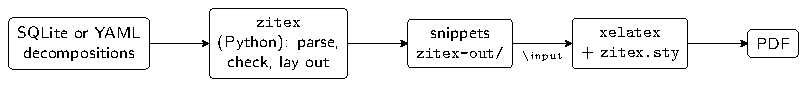
\includegraphics[width=\linewidth]{flow.pdf}
\caption{The workflow. Python writes one self-contained snippet per character and style, and XeLaTeX includes them.}
\label{fig:flow}
\end{figure}

\paragraph{Views.} The equation view uses only \cmd{text}, \cmd{overset}, \cmd{underbrace} and \cmd{xrightarrow}, so it also works in MathJax. The matrix
and the tree are TikZ pictures with coordinates computed in Python, which allows patterns of any size without a TikZ tree library.

\paragraph{Pictures.} A character has sound, shape and meaning, and the equation view shows only the first and the last. The picture view
(\cmd{zimath}\texttt{[pict]\{字\}}) lays the equation out as one grid: for every part, the pinyin, the character, a short meaning and a picture,
in rows that line up across the parts, so that the pictures share one line and the meanings another. A row that no part fills is left out, and
a part without a picture has an empty cell. A picture is an image file, or else an emoji, or else nothing. XeLaTeX cannot print colour emoji, so an
emoji is drawn into a PNG when the snippets are built. Every picture is set in a box of the same size, which is a setting and not part of the
data. The meaning is the gloss, or else the concept, or else the concept category, or else nothing. Pictures come in named sets
(\cmd{zimath}\texttt{[pict=obs]\{字\}}), so one document can show the same equations with emoji and with oracle bone glyphs.
This view uses images, so it needs XeLaTeX and is not available in MathJax.

\paragraph{Readings.} Which part carries the meaning and which the sound is an interpretation. A character may store several named
\emph{readings}, selected per call with \texttt{reading=}, so that two interpretations can be set in one document without duplicating the data.

\paragraph{Validation.} \texttt{zitex check} reports unknown positions, patterns an operator does not allow, overlapping regions, and a radical placed
at the centre. These are warnings and not errors, because the data being typeset is itself under review.

\paragraph{Fonts.} A component is resolved in a fixed order: an explicit override, the primary font, fallback fonts, an image, and finally a boxed code point
with a warning. Components that have no Unicode code point can therefore be set like any other.

\paragraph{Data.} Decompositions come from YAML files or from a SQLite database. The database is opened read only. \texttt{zitex} derives its own tables from it, and
a hand revision is stored together with what it replaced, so that it can be reverted and is re-applied when the tables are rebuilt.
A Streamlit application reviews and revises decompositions, and generates a PDF for a list of characters.

\section{Example}\label{sec:example}
The commands below make a self-contained folder and typeset three characters.

\begin{verbatim}
zitex setup   -o work/
zitex extract -c 器,藻,佛 -o work/
cd work && xelatex main.tex
\end{verbatim}

The document asks for views with \cmd{zimath}\texttt{\{藻\}}, \cmd{zimatrix}\texttt{\{器\}}, \cmd{zitree}\texttt{\{藻\}}
and \cmd{ziformula}\texttt{\{佛\}}. They give:

\zimath{藻}

\begin{figure}[ht]
\centering
\zimatrix{器}\qquad\zimatrix{佛}
\caption{Zi-Matrices of 器 (four 口 at the corners and 犬 in the centre) and 佛 (亻 and 弗).}
\label{fig:matrix}
\end{figure}

\begin{figure}[ht]
\centering
\resizebox{0.85\linewidth}{!}{\zitree{藻}}
\caption{The decomposition tree of 藻. Leaves are parts that are not decomposed further.}
\label{fig:tree}
\end{figure}

\noindent The matrix keeps the geometry (Figure~\ref{fig:matrix}), and the tree shows the depth (Figure~\ref{fig:tree}): 藻 has four levels, because 澡 and 喿 are decomposed too.
Inline, \cmd{ziformula}\texttt{\{器\}} gives \ziformula{器}\unskip.

\subsection{Sound, shape and meaning}
The picture view adds the third dimension of a character. Each part carries its pinyin above, its meaning below, and a picture under the meaning.
The input is a lexicon entry per character (here the pictures are emoji), the decomposition of the result, and the call in the document:

\begin{verbatim}
# lexicon.yaml
日: {pinyin: rì,   gloss: {en: sun,    zh: 太阳}, pict: <emoji: sun>}
月: {pinyin: yuè,  gloss: {en: moon,   zh: 月亮}, pict: <emoji: moon>}
明: {pinyin: míng, gloss: {en: bright, zh: 明亮}, pict: <emoji: sparkles>}

\zimath[pict]{明}            % English meanings
\zimath[pict,lang=zh]{明}    % Chinese meanings
\end{verbatim}

\noindent Reading 日 + 月 = 明 as \emph{sun} and \emph{moon} making \emph{bright}, and 虫 + 工 = 虹 in the same way, gives:

\paragraph{Emoji as the picture.}
\zimath[pict]{明}
\zimath[pict,lang=zh]{明}
\zimath[pict]{虹}

\noindent The meanings are in English in the first and third equation and in Chinese in the second: the language is a key of the call, and any language
that the lexicon has can be used.

\paragraph{Oracle bone glyphs as the picture.}
Chinese characters began as pictographs, so the picture row can show the ancient form of each part. The glyphs come from the HUST-OBC
dataset of oracle bone characters~\cite{hustobc}, one chosen glyph per character, stored as \texttt{u<hex>.png} files and added to the lexicon as a
second set of pictures, \texttt{pict\_obs}. A call names the set it wants:

\begin{verbatim}
zitex render -i chars.yaml --scan main.tex \
    -x lexicon.yaml -x obs/lexicon.yaml -l en -l zh
\zimath[pict=obs,lang=zh]{明}
\zimath[pict=obs,lang=zh]{虹}
\end{verbatim}

\zimath[pict=obs,lang=zh]{明}
\zimath[pict=obs,lang=zh]{虹}

\noindent The pictures differ from the emoji in what they show. In the glyphs chosen here, 明 is a crescent next to a small box and not a sun and a moon,
and 虹 is an arch with a head at each end. The figures show the data: a modern decomposition and an ancient glyph are separate records, and the
picture row puts them side by side without interpreting either. In the same way the set is optional for each character: a part with no glyph in the set
has an empty cell and is not replaced by an emoji.

\section{Related work and limitations}
The Unicode Standard defines ideographic description characters, and community projects distribute ideographic description sequences
for large character sets~\cite{cjkviids}. These record a character as a string and do not give positions or figures. \texttt{zitex} reads this
form and adds positions per level. Figures are produced with TikZ~\cite{tikz}, and Chinese text with \texttt{xeCJK}~\cite{xecjk}, which \texttt{zitex} builds on.
We did not survey other tools for drawing character decompositions, and a comparison is future work.

The present version has these limits. It needs XeLaTeX, and has not been tried with other engines. The picture view is not available in MathJax, because it
uses images, and a long equation with long meanings can be wider than the page: the width of a meaning and the number of senses shown are settings, and
nothing scales the equation. The oracle bone glyphs are a handful chosen by the author for these examples, and most elemental characters have no chosen glyph yet. The snippet file names are ASCII, which
should work on any file system, but we have only tried Linux. The decomposition database used for development is a first iteration under review:
223 rows of about 6,200 cannot be converted yet, and warnings remain on some characters. Glosses are first senses from a dictionary and are not curated.
We make no claim about the etymology of any character: the figures show the data.

\section*{Acknowledgements}
This work began as a conversation with Google Gemini, and the building, testing and writing phases were assisted by Claude Code of Anthropic. The character decompositions, solution design, and result validation are the author's.

The English glosses are derived from CC-CEDICT (CC BY-SA 4.0)~\cite{cedict} and are attributed in the data. The oracle bone glyph images in
Section~\ref{sec:example} are from HUST-OBC~\cite{hustobc}, which is licensed CC BY-NC 4.0: they may be reused for non-commercial research with
attribution, and are not covered by the MIT licence of the code.

\begin{thebibliography}{9}
\bibitem{gong2025} Wen G. Gong. \emph{A New Exploration into Chinese Characters: from Simplification to Deeper Understanding}. arXiv:2502.19428, 2025.
\bibitem{cjkviids} \emph{cjkvi-ids: Ideographic Description Sequences for CJKV characters}. \url{https://github.com/cjkvi/cjkvi-ids}.
\bibitem{hustobc} Pengjie Wang et al. \emph{An open dataset for oracle bone character recognition and decipherment}. Scientific Data, 2024. arXiv:2401.15365.
\bibitem{cedict} \emph{CC-CEDICT: a Chinese-English dictionary}. \url{https://cc-cedict.org}.
\bibitem{tikz} Till Tantau. \emph{The TikZ and PGF Packages}. CTAN, \url{https://ctan.org/pkg/pgf}.
\bibitem{xecjk} \emph{The xeCJK package}. CTAN, \url{https://ctan.org/pkg/xecjk}.
\end{thebibliography}
\end{document}
